\documentclass[
        12pt,
        openany, %openright,			
        oneside, %twoside,			%% twoside: para frente e verso ao imprimir
        a4paper,			
        english,			
%	french,				%% Idioma adicional 
%	spanish,			%% Idioma adicional 
        brazil			        %% Idioma principal 
        ]{abntbibufjf}

\usepackage{lmodern}						
\usepackage[T1]{fontenc}		
\usepackage[utf8]{inputenc}		%% Para converter automaticamente acentos como digitados. Mude utf8 para latin1 se precisar. 
                                        %% Permite digitar os acentos no teclado normalmente, sem comandos (\'e \`a , etc.).
\usepackage{lastpage}			
\usepackage{indentfirst}		
\usepackage{color}		
\usepackage[alf,abnt-emphasize=bf,abnt-etal-list=0,abnt-etal-text=it]{abntex2cite}	
\usepackage{graphicx}			
\usepackage{microtype} 	



%% -----------------------------------------------------------------------------

%% Obs.: Alguns acentos foram omitidos.

\titulo{Implementando a metodologia lean no desenvolvimento de software} %%Por exemplo, Titulo da tese
% \subtitulo{: subt\'itulo do trabalho}  %% Retirar o primeiro ``%'' desta linha se for utilizar subtitulo. Deixar os dois pontos antes, em ``: subt\'itulo'' . 
\autor{Lucas José Merencia}
\autorR{Merencia, Lucas josé} %%Colocar o sobrenome do autor antes do primeiro nome do autor, separados por ,
\local{Joinville}
\data{2015} %%Alterar o ano se precisar
\orientador[Orientador:]{Andre Vinicius Castoldi} %%Se precisar, troque [Orientador:] por [Orientadora:]
% \coorientador[Coorientador:]{Nome do coorientador } %% Retirar o primeiro ``%'' desta linha se tiver coorientador. Se precisar, troque por [Cooorientadora:]. 
\instituicao{Centro Universitário -- Católica de Santa Catarina}
\faculdade{Instituto de Ci\^encias Exatas} %%Alterar, dentro de chaves {}, se precisar.
\programa{Curso de P\'os\mbox{-Gra}dua\c{c}\~ao em Engenharia de Software} %%Alterar, dentro de chaves {}, se precisar.
\objeto{Monografia}  %%Tese (Doutorado)
\natureza{Monografia  %%Tese
apresentada ao \insereprograma ~do \insereinstituicao ~como requisito parcial para obten\c{c}\~ao do certificado do curso.} %%Trocar Matem\'atica por outro, se precisar.


%% Abaixo, prencher com os dados da parte final da ficha catalografica

\finalcatalog{1. Lean. 2. Metodologia de Desenvolvimento. 3. Engenharia de Sofware. I. Henning, Maurício. Msc.} %% Aqui fica 
% escrito a palavra ``T\'itulo'' mesmo, nao o do trabalho. Se tiver coorientador, os dados ficam depois dos dados 
%% do orientador (II. Sobrenome, Nome do coorientador, coorient.) e antes de ``II. T\'itulo'', o qual passa a ``III. T\'itulo''.

%% ---

\setlength{\parindent}{1.3cm}

\setlength{\parskip}{0.2cm}  

\setlength\afterchapskip{12pt}  

%% Iniciar o documento
\begin{document}

%% ELEMENTOS PRE-TEXTUAIS

%% Capa
\inserecapa

%% Folha de rosto
\inserefolhaderosto


%% Ficha catalografica. AO IMPRIMIR, DEIXAR NO VERSO DA FOLHA DE ROSTO.
\inserecatalog  


%% Folha de aprovacao
\begin{folhadeaprovacao}

  \begin{center}
    {\chapterfont \MakeUppercase{\bfseries \insereautor}}

    \vfill
    \begin{center}
      {\chapterfont \MakeUppercase{\bfseries\inseretitulo \inseresubtitulo}}
    \end{center}
    \vfill
    
    \hspace{.45\textwidth}
    \begin{minipage}{.5\textwidth}
        \inserenatureza
        \\ \\
        \begin{center}COMISSÃO EXAMINADORA \end{center}
         \assinatura{Prof. Msc. \insereorientador \ - Orientador \\ Centro Universitário -- Católica de Santa Catarina} 
      %  \assinatura{Professor Dr. \inserecoorientador \ - Coorientador \\ Universidade Federal de Juiz de Fora}
         \assinatura{Professor Dr. ?? \\ Universidade ???}
         \assinatura{Professor Dr. ?? \\ Universidade ??} 
    \end{minipage}%
    \vfill
   \end{center}
           

%  \assinatura{...} %%RETIRE O % E PREENCHA SE PRECISAR
%  \assinatura{...}
%  \assinatura{...}
\end{folhadeaprovacao}


%% Dedicatoria. OPCIONAL. Retirar o ``%'' de cada das 4 linhas abaixo, caso queira.
% \begin{dedicatoria} \vspace*{\fill} \centering \noindent
%   \textit{ Dedico este trabalho ... (opcional)} 
%   \vspace*{\fill}
% \end{dedicatoria}


%% Agradecimentos. OPCIONAL. CASO SEJA BOLSISTA, INSERIR OS DEVIDOS AGRADECIMENTOS.
%\begin{agradecimentos}

%Este trabalho é decicado à minha família, meus amigos, meu orientador e a Católica de Santa Catarina. 

%\end{agradecimentos}

%% Epigrafe. OPCIONAL
% \begin{epigrafe}
%     \vspace*{\fill}
% 	\begin{flushright}
% 		``Texto em que o autor apresenta uma cita\c{c}\~ao, seguida de autoria, relacionada com a                       
%   mat\'eria tratada no corpo do trabalho'' \\
% (ASSOCIA\c{C}\~AO BRASILEIRA DE NORMAS T\'ECNICAS, 2011, p. 2) \\
%   A ep\'igrafe elaborada conforme NBR 10520 (Ep\'igrafe - Opcional)
% 	\end{flushright}
% \end{epigrafe}


%% RESUMOS

%% Resumo em Portugu^es. OBRIGATORIO.
\setlength{\absparsep}{18pt} 
\begin{resumo}
 ... Resumo
\textbf{Palavras-chave}: Alguma Palavra-chave, Engenharia de Software. %finalizadas por ponto e inicializadas por letra maiuscula.

\end{resumo}
 
 
%% Resumo em Ingle^s
\begin{resumo}[ABSTRACT]
 \begin{otherlanguage*}{english}
 ... Abstract
\textbf{Keywords}: Some Keyword, Software Engineering.
 \end{otherlanguage*}
\end{resumo}

%% Seguindo o mesmo modelo acima, pode-se inserir resumos em outras linguas. 

%% Lista de ilustracoes. OPCIONAL.
\pdfbookmark[0]{\listfigurename}{lof}
\listoffigures*
\cleardoublepage


%% Lista de tabelas. OPCIONAL. Retire o ``%'' de cada das 3 linhas seguintes, caso queira.
\pdfbookmark[0]{\listtablename}{lot}
\listoftables*
\cleardoublepage

%% Lista de abreviaturas e siglas. OPCIONAL
\begin{siglas} %%ALTERAR OS EXEMPLOS ABAIXO, CONFORME A NECESSIDADE
  \item[SIGLA] Siglas vão aqui
\end{siglas}

%% Lista de simbolos. OPCIONAL
% \begin{simbolos} %%ALTERAR OS EXEMPLOS ABAIXO, CONFORME A NECESSIDADE
%   \item[$ \forall $] Para todo
%   \item[$ \in $] Pertence
%  \end{simbolos}

 
%% Sumario
\pdfbookmark[0]{\contentsname}{toc}
\tableofcontents*
\cleardoublepage

%% ----------------------------------------------------------

%% ELEMENTOS TEXTUAIS

\textual
\pagestyle{simple}   

\setcounter{page}{1}
\chapter{INTRODU\c{C}\~AO}  %%Nesta linha, dentro de { }, digita-se em CAIXA ALTA, como apresentado aqui
\label{chap:01}

O \textit{software} está inserido em praticamente todos os aspectos de nossas vidas, podendo colaborar para a otimização da linha de produção de industrias, melhorar a gestão de empresas ou até mesmo mudar a forma como as pessoas se relacionam. Diante desta grande demanda, o \textit{software} e todos os artifícios envolvidos em seu desenvolvimento precisam ser constantemente aperfeiçoados, desta forma, a engenharia de \textit{software} surgiu com o objetivo de aplicar princípios de engenharia na especificação, no desenvolvimento e na manutenção de \textit{software}.

A grande demanda para construções de \textit{softwares} cada vez mais complexos e com mais funcionalidade, acarretou em projetos extensos, com bases de códigos enormes, que desencadeiam diversos problemas para o gerenciamento, por exemplo, erros de estimativa, custos elevados e até mesmo desgastes emocionais e desmotivação dos engenheiros envolvidos. Para minimizar os problemas de projetos extensos, a engenharia de \textit{software} possui o conceito de modularidade, nele é enfatizado que o \textit{software} modular pode ser melhor gerenciado que o monolítico. Além disso, a modularização possibilita que o \textit{software} seja planejado mais facilmente e que os custos para manutenção sejam reduzidos.

Diferente da abordagem monolítica o desenvolvimento de \textit{software} baseado em \textit{microservices} visa construir vários \textit{softwares} menores, com propósitos específicos, que se comunicam trocando informações para resolver problemas complexos. Basicamente neste modelo a modularização é intensificada visando simplificar ao máximo a complexidade dos projetos. Entretanto muitas vezes o projeto não se iniciou seguindo o modelo de \textit{microservices}, desta forma, muitas vezes os \textit{microservices} são extraídos de um \textit{software} maior, em muitos casos de um monolito.

Este trabalho visa propor um modelo para extração de \textit{microservice} de um \textit{software} monolítico, baseado em um cenário real de uma empresa de tecnologia, que está em amplo crescimento, e que por possuir um \textit{software} monolítico, enfrenta vários problemas ocasionados pelo modelo de arquitetura de \textit{software} adotado.

\section{OBJETIVOS}

O objetivo deste trabalho é propor um modelo de arquitetura de \textit{software} que possibilite a extração gradativa de \textit{microservices} de um \textit{software} monolítico, sem que haja a necessidade de reescrever toda a aplicação no novo modelo, ou seja, deverá ser possível além de evoluir a arquitetura de \textit{software} dando suporte a evolução constante do produto, desta forma, possibilitando que novas funcionalidades sejam adicionadas e mantidas.

\section{JUSTIFICATIVA}

Na ContaAzul, empresa localizada em Joinville, todo o \textit{software} (ContaAzul) está centralizado em um único projeto e cada um dos vários times de desenvolvimento que a empresa possui é responsável por um conjunto de funcionalidades, desta forma todos os times trabalham dando manutenção e inserindo novas funcionalidades na mesma aplicação monolítica.

Tendo mais de 50 engenheiros de  o \textit{software}, diariamente executando o processo de desenvolvimento na mesma grande base de código do ContaAzul, fica evidenciado os problemas da aplicação monolítica, refletidos em atrasos para finalizações de tarefas do processo de desenvolvimento. A Figura \ref{fig:01} apresenta o processo de desenvolvimento atual adotado pelos times da ContaAzul.

\begin{figure}[hb]
	\begin{center}
		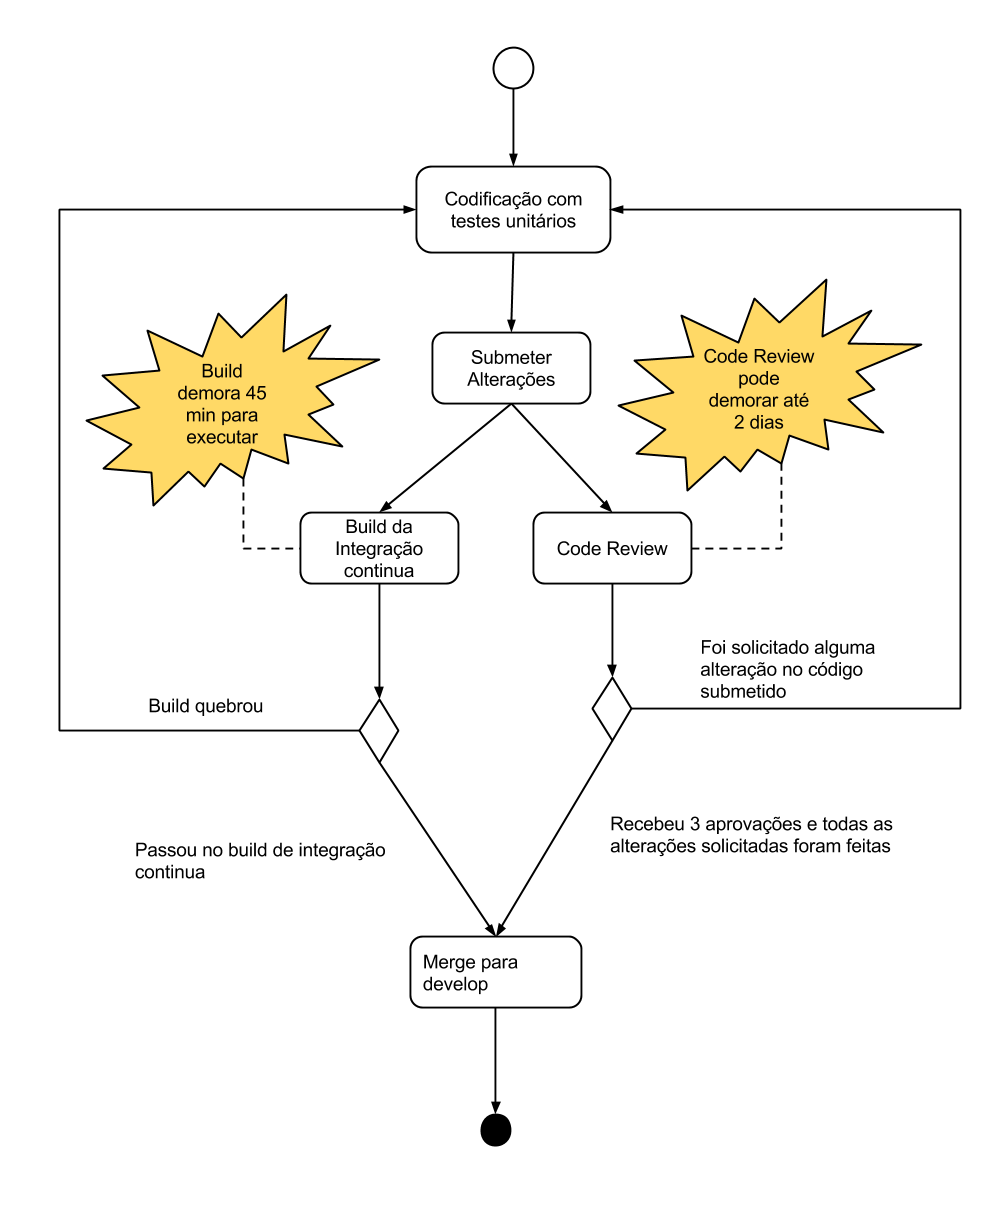
\includegraphics[width=12cm]{assets/processo_desenvolvimento.png}
		\caption{Processo de Desenvolvimento dos Times da ContaAzul}
		\label{fig:01}
	\end{center}
\end{figure}

Na Figura \ref{fig:01} são evidenciado os 2 problemas mais custosos do processo, foi decidido pelo time de engenharia da empresa que o custo para alteração do processo e readequação de todo o modelo de trabalho, não resolveria o causa rais dos problemas, o \textit{software} monolítico.

Desta forma, pensando a logo prazo, foi identificado que a migração para um modelo de \textit{microservices} poderia ser uma proposta melhor para solucionar os problemas apontados.

\section{ESTRUTURA DO TRABALHO}

// TODO: Definir a estrutura do trabalho 


\chapter{FUNDAMENTAÇÃO TEÓRICA}
\label{chap:02}

Neste capítulo são abordadas as tecnologias e conceitos necessários para a compreensão e embasamento do objetivo proposto.

\section{MICROSERVICES}

\section{AUTOMAÇÃO DE TESTES}

Para garantir a qualidade dos \textit{microservices}, os mesmos devem ser amplamente testados. Normalmente no processo de desenvolvimento de \textit{software} existe uma fase de testes, que após a codificação, visa a garantia de qualidade e que o código gerado esteja funcionando como o esperado. Entretanto, com o crescimento do \textit{software} e com o aumento de sua complexidade, tornam a etapa de testes custosas. Dessa forma, a automação de testes surge como uma alternativa para minimizar os custos dessa etapa e agilizar o processo de desenvolvimento sem lesar a qualidade. Segundo \citeonline{bernardo2008importancia}, a grande vantagem desta abordagem, é que todos os casos de teste podem ser facilmente e rapidamente repetidos a qualquer momento e com pouco esforço.

De modo geral os testes automatizados são \textit{scripts} simples que exercitam funcionalidades do sistema e fazem verificações automáticas nos efeitos colaterais obtidos. A reprodutibilidade dos testes permite simular identicamente e inúmeras vezes situações específicas, garantindo que passos importantes não serão ignorados por falha humana e facilitando a identificação de um possível comportamento não desejado. \cite{bernardo2008importancia}

Com a finalidade de garantir a qualidade dos \textit{microservices} e garantir o contrato para comunicação entre os serviços, foram utilizados 2 tipos de testes automatizados: Testes unitários e testes de integração.

\subsection{Testes Unitários}

Para \citeonline{pressman}, um teste unitário focaliza o esforço de verificação na menor unidade de projeto de \textit{software}. Deste modo, por testar pequenas partes isoladas do \textit{software} os testes unitários podem ser de grande valor para a garantia de qualidade do código. Além disso, segundo \citeonline{bernardo2008importancia}, o teste de uma unidade é o tipo mais importante de teste para a grande maioria das situações, já que é ele que deve testar se um algoritmo faz o que deveria ser feito e garantir que o código encapsulado por uma unidade deve produzir o efeito colateral esperado.

\subsection{Testes de Integração}

\section{INTEGRAÇÃO CONTINUA}

\section{AUTOMAÇÃO DE DEPLOY}
\chapter{MATERIEAIS E MÉTODOS}
\label{chap:03}

// TODO

\postextual


\bibliography{referencias}

%% Referencias. LISTAR EXATAMENTE AS CITADAS NO TRABALHO.
% \begin{thebibliography}{99}

% %% ALGUNS EXEMPLOS ABAIXO

% \bibitem{Ferrari2003} FERRARI, M. Amplia\c{c}\~ao e refor\c{c}o do vocabul\'ario em l\'ingua estrangeira atrav\'es da narra\c{c}\~ao e 
% da leitura de hist\'orias infanto-juvenis. \textit{Letras Hoje}, Porto Alegre, v. 39, n. 3, p. 73-90, set. 2003.

% \bibitem{CalcB} FLEMMING, D. M.; GON\c{C}ALVES, M. B. \textit{C\'alculo B.} S\~ao Paulo: Makron Books, 2007.

% \bibitem{Figueiredo96} FIGUEIREDO, D. G. \textit{An\'alise I.} Rio de Janeiro: Livros T\'ecnicos e Cient\'ificos, 1996.

% \end{thebibliography}




%% Apendices

% \begin{apendicesenv}

% \chapter{T\'itulo do Primeiro Ap\^endice}

% ``Texto ou documento elaborado pelo autor, a fim de complementar sua argumenta\c{c}\~ao, 
% sem preju\'izo da unidade nuclear do trabalho''
% (ASSOCIA\c{C}\~AO BRASILEIRA DE NORMAS T\'ECNICAS, 2011, p. 6).

% ``Elemento opcional. Deve ser precedido da palavra \textbf{AP\^ENDICE}, identificado por letras mai\'usculas 
% consecutivas, travess\~ao e pelo respectivo t\'itulo. Utilizam-se letras mai\'usculas dobradas, 
% na identifica\c{c}\~ao dos ap\^endices, quando esgotadas as letras do alfabe\-to.''
% (ASSOCIA\c{C}\~AO BRASILEIRA DE NORMAS T\'ECNICAS, 2011, p. 13)
% \newline
% EXEMPLO:
% \begin{center}
% \textbf{AP\^ENDICE A - Avalia\c{c}\~ao num\'erica de c\'elulas inflamat\'orias}
% \end{center}


% \chapter{Segundo Ap\^endice}
% Texto do Segundo Ap\^endice 
% \end{apendicesenv}

%% Anexos

% \begin{anexosenv}

% \chapter{T\'itulo do Primeiro Anexo}
% ``Texto ou documento n\~ao elaborado pelo autor, que serve de fundamenta\c{c}\~ao, 
% comprova\c{c}\~ao e ilustra\c{c}\~ao''
% (ASSOCIA\c{C}\~AO BRASILEIRA DE NORMAS T\'ECNICAS, 2011, p. 9).

% ``Elementos opcional. Deve ser precedido da palavra \textbf{ANEXO}, identificado por letras mai\'usculas 
% consecutivas, travess\~ao e pelo respectivo t\'itulo. Utilizam-se letras mai\'usculas dobradas, 
% na identifica\c{c}\~ao dos anexos, quando esgotadas as letras do alfabeto.''
% (ASSOCIA\c{C}\~AO BRASILEIRA DE NORMAS T\'ECNICAS, 2011, p. 6).
% \newline
% EXEMPLO: 
% \begin{center}
% \textbf{ANEXO A - Representa\c{c}\~ao gr\'afica da contagem de c\'elulas inflamat\'orias presentes
% nas caudas em regenera\c{c}\~ao - Grupos de controle I (Temperatura)}
% \end{center}


% \chapter{T\'itulo do Segundo Anexo}
% Texto do Segundo Anexo


% \end{anexosenv}

%%% ---
\end{document}
